\begin{abstract}
Zero-shot reinforcement learning (RL) algorithms aim to learn a family of policies from a reward-free dataset, and recover optimal policies for any reward function directly at test time. Naturally, the quality of the pretraining dataset determines the performance of the recovered policies across tasks. However, pre-collecting a relevant, diverse dataset without prior knowledge of the downstream tasks of interest remains a challenge. 
In this work, we study \textit{online} zero-shot RL for quadrupedal control on real robotic systems, building upon the Forward-Backward (FB) algorithm. We observe that undirected exploration yields low-diversity data, leading to poor downstream performance and rendering policies impractical for direct hardware deployment. Therefore, we introduce ~\method, an online zero-shot RL algorithm that combines an unsupervised behavior exploration strategy with a regularization critic. \method promotes exploration by maximizing the entropy of the achieved behavior distribution. Additionally, a regularization critic shapes the recovered policies toward more natural and physically plausible behaviors. 
We empirically demonstrate that \method achieves and improved performance compared to other exploration strategies in a range of simulated downstream tasks, and that it renders natural policies that can be seamlessly deployed to hardware without further finetuning. Videos and code available on our \href{https://math-286-pro.github.io/FB-MEBE-Web/}{website}.

\begin{figure}[H]
    \centering
    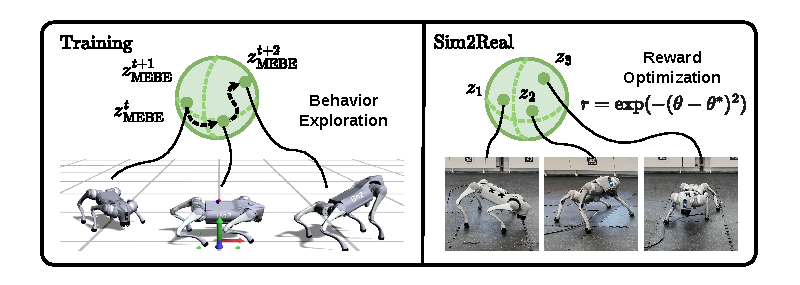
\includegraphics[width=1.0\linewidth]{figure/FB-Teaser.pdf} 
    \caption{\method improves behavior exploration by maximizing the behavior entropy during training. With the regularizer critic, \method achieves zero-shot hardware deployment by optimizing reward at inference time.}
    \label{fig:teaser}
\end{figure}
\end{abstract}

